%%%%%%%%%%%%%%%%%%%%%
%% Configuração %%
%%%%%%%%%%%%%%%%%%%%%

\section{Introdução}
Antes de utilizar o SAEC de fato, é necessário passar por uma etapa de configuração do sistema. Acessando o sistema pela primeira vez com o endereço configurado no \textit{Virtual Host} do Apache, a página mostrada deve ser de login, assim como a figura \ref{fig:entrada}. Inicialmente, o usuário \textit{default} do sistema possui login "administrator" e senha "icpedu.

\begin{figure}[h]
     \centering
     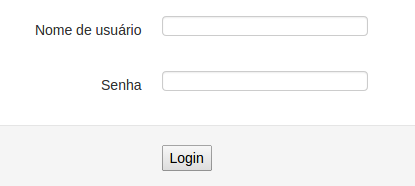
\includegraphics[scale=0.5]{images/entrada.png}
     \caption{Entrada no sistema}
     \label{fig:entrada}
\end{figure}

%%%%%%%%%%%%%%%%%%%%%

\section{Dados do Admin}
A primeira etapa do processo de configuração é a alteração do dados do administrador do sistema. Como trata-se de um ambiente de desenvolvimento, podemos utilizar dados falsos. Neste ponto, a "senha do usuário", que se refere à senha do usuário logado, ainda é a senha padrão, mas tenha em mente que a partir do momento que o formulário for submetido, o nome de usuário e senha escolhidos passarão a ser as novas credenciais do usuário administrador e serão exigidas nas próximas etapas de configuração. O usuário \textit{default} deixará de existir.

\begin{figure}[h]
     \centering
     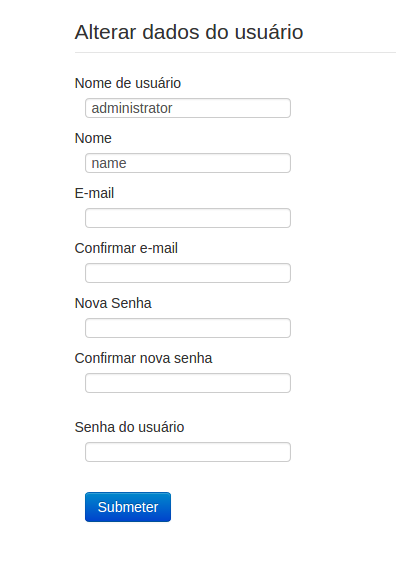
\includegraphics[scale=0.48]{images/inicioadmin.png}
     \caption{Dados do Admin}
     \label{fig:inicioadmin}
\end{figure}

%%%%%%%%%%%%%%%%%%%%%

\section{Restauração de Backup}
Em seguida, é dada a opção de inicializar o SAEC a partir de um backup previamente feito de outra instância da aplicação. É uma função muito útil em fase de testes de usuário, quando, por exemplo, for necessário limpar o banco de dados e reconfigurar o SAEC, ou quando a funcionalidade que deseja-se testar está incluída nos passos de configuração inicial do sistema. Caso seja recuperado algum backup, a aplicação é configurada automaticamente com as informações contidas nele, e a etapa de configuração é encerrada. Caso contrário, segue-se para o próximo passo.
    
    \begin{figure}[h]
     \centering
     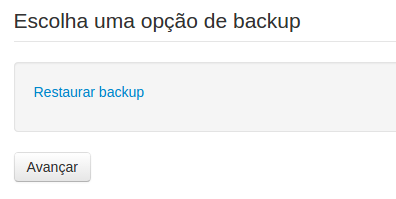
\includegraphics[scale=0.6]{images/opcaobackup.png}
     \caption{Restauração de Backup}
     \label{fig:opcaobackup}
\end{figure}

%%%%%%%%%%%%%%%%%%%%%

\section{Armazenamento de Chave}
Deve ser escolhido qual será o tipo de armazenamento utilizado para guardar a chave privada da Autoridade Certificadora do SAEC. Em ambientes de desenvolvimento, normalmente utilizamos "Chave em disco", embora seja necessário em alguns momentos, principalmente para testes, utilizar a opção "Módulo de Hardware Seguro", visto que em ambiente de produção é a opção que muito provavelmente deverá ser escolhida.
    
    \begin{figure}[h]
     \centering
     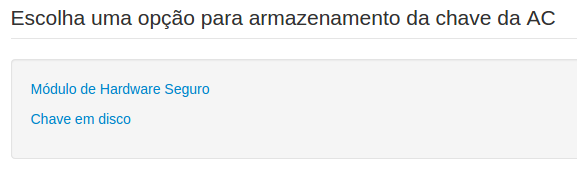
\includegraphics[scale=0.6]{images/armazenachave.png}
     \caption{Opção de armazenamento de chave}
     \label{fig:armazenachave}
\end{figure}

\subsection{Configuração do MSC}
Caso seja escolhida a opção que utiliza um Módulo de Segurança Criptográfico (MSC), é necessário salvar as configurações de acesso à ele, para que seja possível utilizar a chave privada da AC sempre que necessário.

TODO: explicar como se preenche esse form
    
    \begin{figure}[h]
     \centering
     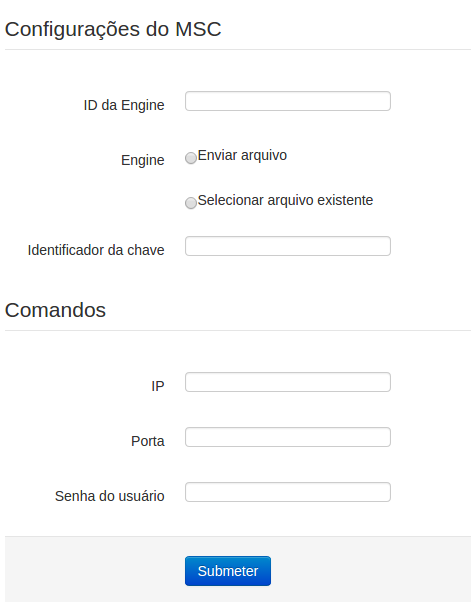
\includegraphics[scale=0.5]{images/confighsm.png}
     \caption{Configuração do MSC}
     \label{fig:confighsm}
\end{figure}

%%%%%%%%%%%%%%%%%%%%%

\section{Emissão do Certificado da AC}
\subsection{Criação da Requisição de Certificado}
TODO:refactor + printscreen

    Depois de configurá-lo, você será redirecionado para a página de criação de requisição para o seu sistema de emissão de certificados ICPEdu. Esta requisição deve ser aprovada por uma Autoridade Certificadora superior, que irá gerar um certificado para o sistema. 


\subsection{Emissão do Certificado}
TODO: guia para instalar SGCI na própria máquina e emitir certificado
    
    \begin{figure}[h]
     \centering
     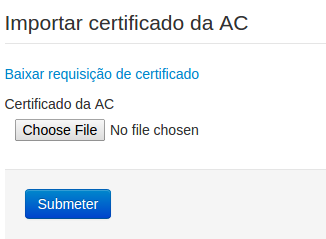
\includegraphics[scale=0.6]{images/importacertAC.png}
     \caption{Importação de certificado}
     \label{fig:reqcert}
\end{figure}


%%%%%%%%%%%%%%%%%%%%%

\section{Configuração de Certificado}
TODO: explain
    
    \begin{figure}[h]
     \centering
     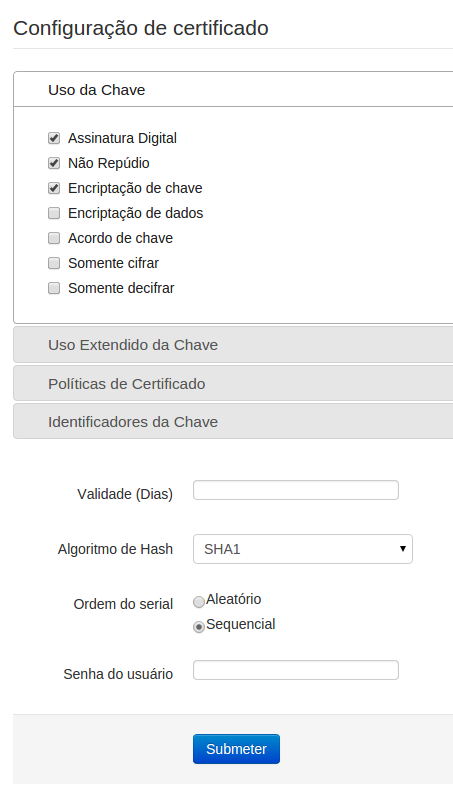
\includegraphics[scale=0.5]{images/configcertificado.png}
     \caption{Configuração do certificado}
     \label{fig:configcertificado}
\end{figure}

%%%%%%%%%%%%%%%%%%%%%

\section{Whitelist}
TODO: explain + printscreen

%%%%%%%%%%%%%%%%%%%%%

\section{Federação}
TODO:explain
    
    ... é selecionar a federação a qual o seu sistema pertence. É possível selecionar a Comunidade Acadêmica Federada (CAFe) ou a Chimarrão. Pode-se ainda escolher outra federação não listada, e neste caso deve-se fornecer as URLs da mesma.
    
%%%%%%%%%%%%%%%%%%%%%
    
\section{Registro de Operador}
TODO:explain
    
    \begin{figure}[h]
     \centering
     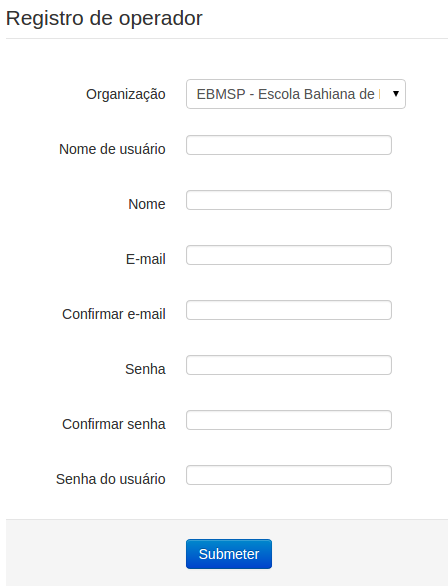
\includegraphics[scale=0.5]{images/inicioregistroop.png}
     \caption{Registro de operador}
     \label{fig:inicioregop}
\end{figure}

TODO:decidir sobre deixar ou não figura da página inicial...
    
    \begin{figure}[h]
     \centering
     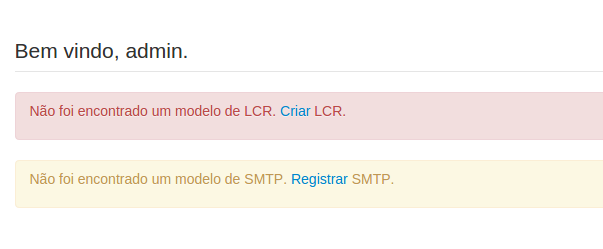
\includegraphics[scale=0.5]{images/pendencias.png}
     \caption{Tarefas pendentes}
     \label{fig:pendencias}
\end{figure}